\documentclass{book}
\usepackage{commeunjeustyle}
\begin{document}
\begin{center}
\begin{Large}
Activité d'introduction
\end{Large}
\end{center}
Pour attirer les clients, un casino propose un nouveau jeu : le croupier lance simultanément 2 dés et calcule leur somme,
\begin{itemize} 
\item si la somme est égale à 2 ou 12, le joueur gagne 2 euros,
\item si la somme est égale à 7, le casino gagne 1 euro,
\item dans les autres cas, c'est nul (le joueur gagne 0 euro).  
\end{itemize}
Un client du casino dit "Comme le joueur a deux fois plus de nombres gagnants et de gains que la banque, ce jeu est favorable au joueur". Êtes-vous du même avis ?

\subsubsection*{Correction d'élève 1} 
Nombre de possibilités avec 2 dés :
\begin{itemize}
\item  toutes,  36 façons car 6.6=36
\item Pour faire 2 ou 12, 2 façons car 1+1=2 et 6+6=12
\item pour faire 7, 6 façons car 1 + 6, 2 + 5, 3 + 4, 4 + 3, 5 + 2 et  6 + 1  
\end{itemize}
On a donc $\frac{2}{36}=\frac{1}{18}$, soit 1 chance sur 18 de gagner et $\frac{6}{36}=\frac{3}{18}$, soit 3 chances sur 18 de perdre.\\
On gagne 2 euros et on perd 1 euro d'où  $2.\frac{1}{18}<1.\frac{3}{18}$ donc le jeu est favorable au casino.

\subsubsection*{Correction d'élève 2}
J'ai simulé 200 parties sur un tableur. J'ai cumulé les gains/pertes, soit \[
\overbrace{(+2)}^{\text{première partie}}+\overbrace{(-1)}^{\text{deuxième partie}}+\overbrace{(-1)}^{\text{troisième partie}}+\dots+\overbrace{(+2)}^{\text{200-ième partie}}\] ce qui m'a donné $-12$ euros.  Donc le jeu est favorable au casino.   

\subsubsection*{Note du professeur} L'élève 1 a utilisé l'approche modélisation des probabilités avec un manque de formalisme. Par exemple, il a écrit "pour faire 7, 6 façons car 1+6,...,6+1". Cependant, 1+6 et 6+1 représente un unique nombre, soit une unique façon, car 1+6=6+1=7. On comprend que le résultat du premier dé est représenté par le nombre à gauche du + et le second à droite.\\
L'élève 2 a utilisé l'approche expérimental de la statistique. Cependant, une autre réalisation aurait pu donné un résultat avec un signe différent (donc une autre conclusion !) car le nombre de parties est faible. La programmation sur un ordinateur aurait permis de simuler un plus grand nombre de parties.\\
Le but des deux prochains paragraphes  est de fournir une compréhension synthétique de l'approche probabiliste et de l'approche fréquentiste avec en fil rouge l'exemple de ce jeu.  



\subsubsection*{Modélisation } L'approche probabiliste consiste à construire un cadre à  cette expérience aléatoire. On définit :
\begin{enumerate}
\item l'\defi{univers}, $\Omega$, l'ensemble de toutes les issues qui peuvent être obtenues au cours d'une expérience aléatoire.\\ 
Dans le jeu, une \defi{issue}, $\omega$, est le couple\footnote{Dans la notation couple, l'ordre est déterminé. Par exemple si $i$ et $j$ sont distincts, le couple $(i, j)$ est distinct du couple $(j, i)$.} de deux dés $(i,j)$ avec $i,j\in\{1,2,\dots,6\}$ et l'univers est : 
\[
\begin{array}{rl}
\Omega=&      \{(i,j): i,j\in\{1,2,\dots,6\}  \}\\
\Omega=&\{(1,1),(1,2),\dots, (1,6),(2,1),(2,2),\dots (2,6),\dots\dots, (6,5),(6,6)\}
\end{array}.
\]
\item  la \defi{tribu}, $\mathcal{A}$, l'ensemble de tous les événements possibles. Un \defi{événement} est un ensemble dont les éléments sont des issues possibles. L'événement élémentaire, $\{\omega\}$, est constitué d'une unique issue $\omega$.\\
Pour le jeu, la tribu est l'ensemble des parties de l'univers, c'est à dire  l'ensemble des sous-ensembles de cet ensemble. En particulier, il y a ces deux événements :
\begin{itemize}
\item "Gagner : obtenir 2 ou 12"=$\{(1,1),(6,6)\}$,
\item "Perdre : obtenir 7 "=$\{(1,6),(2,5),(3,4),(4,3),(5,2),(6,1)\}$.
\end{itemize} 
\item la \defi{probabilité},  une fonction  associant une valeur entre 0 et 1, afin de représenter la chance qu'un événement se réalise.\\
Pour le jeu, comme chaque dé est équilibré, c'est-à-dire que chaque face à la même chance d'apparaitre, les événements élémentaires, correspond aux uniques issues, sont équiprobables,   soit une probabilité : $\mathbb{P}((i,j))=\frac{1}{36} $.  L'arbre de probabilité ci-dessous permet de justifier cette hypothèse : 
\begin{center}
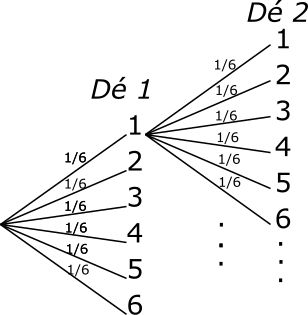
\includegraphics[scale=0.5]{arbre.png}
\end{center}
 On a :    
\begin{itemize}
\item $\mathbb{P}(\text{"Gagner : obtenir 2 ou 12"})=\frac{\text{nombre d'issues de l'événement}}{\text{nombre d'issues de l'univers}}=\frac{2}{36}=\frac{1}{18}$, soit 1 chance sur 18,
\item $P(\text{"Perdre : obtenir 7 ""})=\frac{6}{36}=\frac{3}{18}$, soit 3 chances sur 18.
\end{itemize}
\item  la \defi{variable aléatoire}, une fonction définie depuis l'univers vers un ensemble donné de valeurs dont on déterminera la probabilité.\\ 
Pour le jeu, la variable aléatoire, $X$, représente le gain obtenu (-1 si on perd, 0 nul et 2 si on gagne) en fonction d'une issue :
\begin{center}
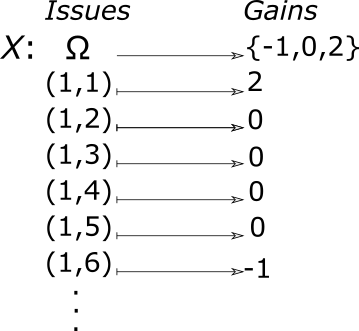
\includegraphics[scale=0.5]{va.png}
\end{center}
La loi de probabilité d'une variable aléatoire est la probabilité d'obtenir une valeur $P(X=x)=P(X^{-1}(\{x\}))$ où $X^{-1}(\{x\}$ est l'image réciproque de $x$ par la fonction $X$,  soit toutes les issues donnant la valeur $x$.\\
Pour le jeu, la probabilité de gain est :
\begin{itemize}
\item  2 euros : $P(X=2)=P( \{(1,1),(6,6)\})=\frac{1}{18}$,
\item  -1 euro : $P(X=-1)=P( \{(1,6),(2,5),(3,4),(4,3),(5,2),(6,1)\})=\frac{3}{18}$,
\item  0 euro :  $P(X=0)=\frac{14}{18}$.
\end{itemize}
\item l'\defi{espérance} d'une variable aléatoire,  une moyenne pondérée par les probabilités d'apparition de chaque valeur, soit intuitivement, la valeur que l'on s'attend à trouver, en moyenne, si l'on répète un grand nombre de fois la même expérience aléatoire.\\
Pour le jeu, l'espérance est : 
\[
\begin{array}{rl}
E[X]=&(-1).P(X=-1) + 0.P(X=0)+2.P(X=2)\\
E[X]=&-1.\frac{3}{18}+ 0.\frac{14}{18}+ 2.\frac{1}{18}\\
E[X]=&-\frac{1}{18}.
\end{array}
\]
\end{enumerate}
En conclusion, le joueur perd en moyenne $\frac{1}{18}$ à chaque partie donc le jeu est favorable au casino.



\subsubsection*{Expérimental} L'approche fréquentiste consiste à réaliser cette expérience aléatoire un grand nombre fois en calculant nos gains cumulés. On représente par :
\begin{itemize}
\item $\omega$  la réalisation de l'élève 2,
\item $X_1$ les gains de la première partie ($X_1(\omega)$ sont les gains de la première partie pour l'élève 2, soit $+2$),
\item $X_2$ les gains de la seconde partie ($X_2(\omega)$ sont les gains de la seconde partie pour l'élève 2, soit $-1$),
\item ... 
\item $X_{200}$ de la 200-ième partie.
\end{itemize}
On note $S_n$ les gains/pertes cumulés après $n$ parties d'où \[S_n=X_1+X_2+\dots+X_n.\]
D'après la correction de l'élève 2, an a :
\[
\begin{matrix}
S_{200}(\omega)=&\overbrace{X_1(\omega)}^{\text{première partie}} &+ & \overbrace{X_2(\omega)}^{\text{seconde partie}} &+&\dots&+&\overbrace{X_{200}(\omega)}^{\text{200-ième partie}}\\
S_{200}(\omega)=&(+2)&+& (-1)&+&\dots&+&(+2)\\
S_{200}(\omega)=&&-12
\end{matrix}
\]
On normalise les gains/pertes cumulés par le nombre de partie afin d'avoir un estimateur du gain moyen . On note, $\overline S_n$, l'estimateur du gain/perte moyen :
\[
\begin{matrix}
\overline S_n = & \frac{S_n}{n}\\
\\
\overline S_n = & \frac{X_1+X_2+\dots+X_n}{n}
\end{matrix}
\]
$\overline S_n$ est un estimateur du gain moyen. D'après la loi forte des grands nombre, $\overline S_n$ converge presque surement vers $E\left[X\right]$

\[
P\left(\omega\in\Omega\ \left|\ \lim_{n}\overline S_n(\omega)=E\left[X\right]\right.\right)=1.
\] 
Cet théorème permet de justifier la cohérence entre les deux approches.  


La programmation nous permet de simuler cette expérience aléatoire pour un $n$ grand. Voici le code dans le langage Python : 
\lstinputlisting[language=Python]{jeu.py.txt}
Pour une réalisation, nous obtenons la valeur $-0,05535$ qui est une bonne approximation du gain moyen égale $\frac{1}{18}=0,0555...$ trouvé dans l'approche modélisation.
    

\end{document}
